 %%%%%%%%%%%%%%%%%%%%%%%%%%%%%%%%%%%%%%%%%%%%%%%%%%%%%%%%%%%%%%%%%%%%%%%%%%%%%
%	e-Yantra, IIT-Bombay

%	Document Author: Akshit Gandhi
%	Date: 7-June,2016
%	Last Editted by: Akshit
%   Date Last updated: 16-06-2016 

%%%%%%%%%%%%%%%%%%%%%%%%%%%%%%%%%%%%%%%%%%%%%%%%%%%%%%%%%%%%%%%%%%%%%%%%%%%%%

\documentclass[11pt,a4paper]{article}
\usepackage{float}
\usepackage{graphicx}
\usepackage{hyperref}
\usepackage{float}
\title{Calibrating the APM}
\author{Akshit Gandhi}
\date{\today}

\begin{document}
	\maketitle
	\newpage
	\tableofcontents
	\newpage
	\section{Objective}
	Topic: Calibrating the APM 2.6/2.5
		In this tutorial we will learn to how to calibrate our APM flight controller. We will be going into details of each step.
	\section{Prerequisites}
	 It's better if you first go through the official documentation on ardupilot's website. The link is: \url{http://ardupilot.org/copter/index.html}, it will be beneficial also for this tutorial and also for later tutorials.
	\section{Hardware Requirement}
	 Drone or Quadcopter, USB cable, a Computer.
	\section{Calibration Process}
	 So, now we start with the process of calibrating the APM. \textbf{Note:} There is are lot's of improvement going on with the APM firmwares and with the associated softwares, so it is advised that you use a more latest software and firmware as it is a refinement of the previous version, but at the time we were working on this project we found that the latest firmware for APM-2.6 was ACv3.3.3 but no-where we could find this firmware so we switched to a previous firmware which was ACv3.2.1 and also to ACv3.1.5.
	 \paragraph{•}We also found out that the latest version of Mission Planner should support for the latest version of the APM firmware, so we had to switch to a more previous version of the Mission Planner software. Mission Planner is software which will help us throughout the calibration process and many more times as we will see later. The Mission Planner Software we are using is V1.3.30 which should look something like this: 
	 \begin{figure}[H]
	 	\centering
		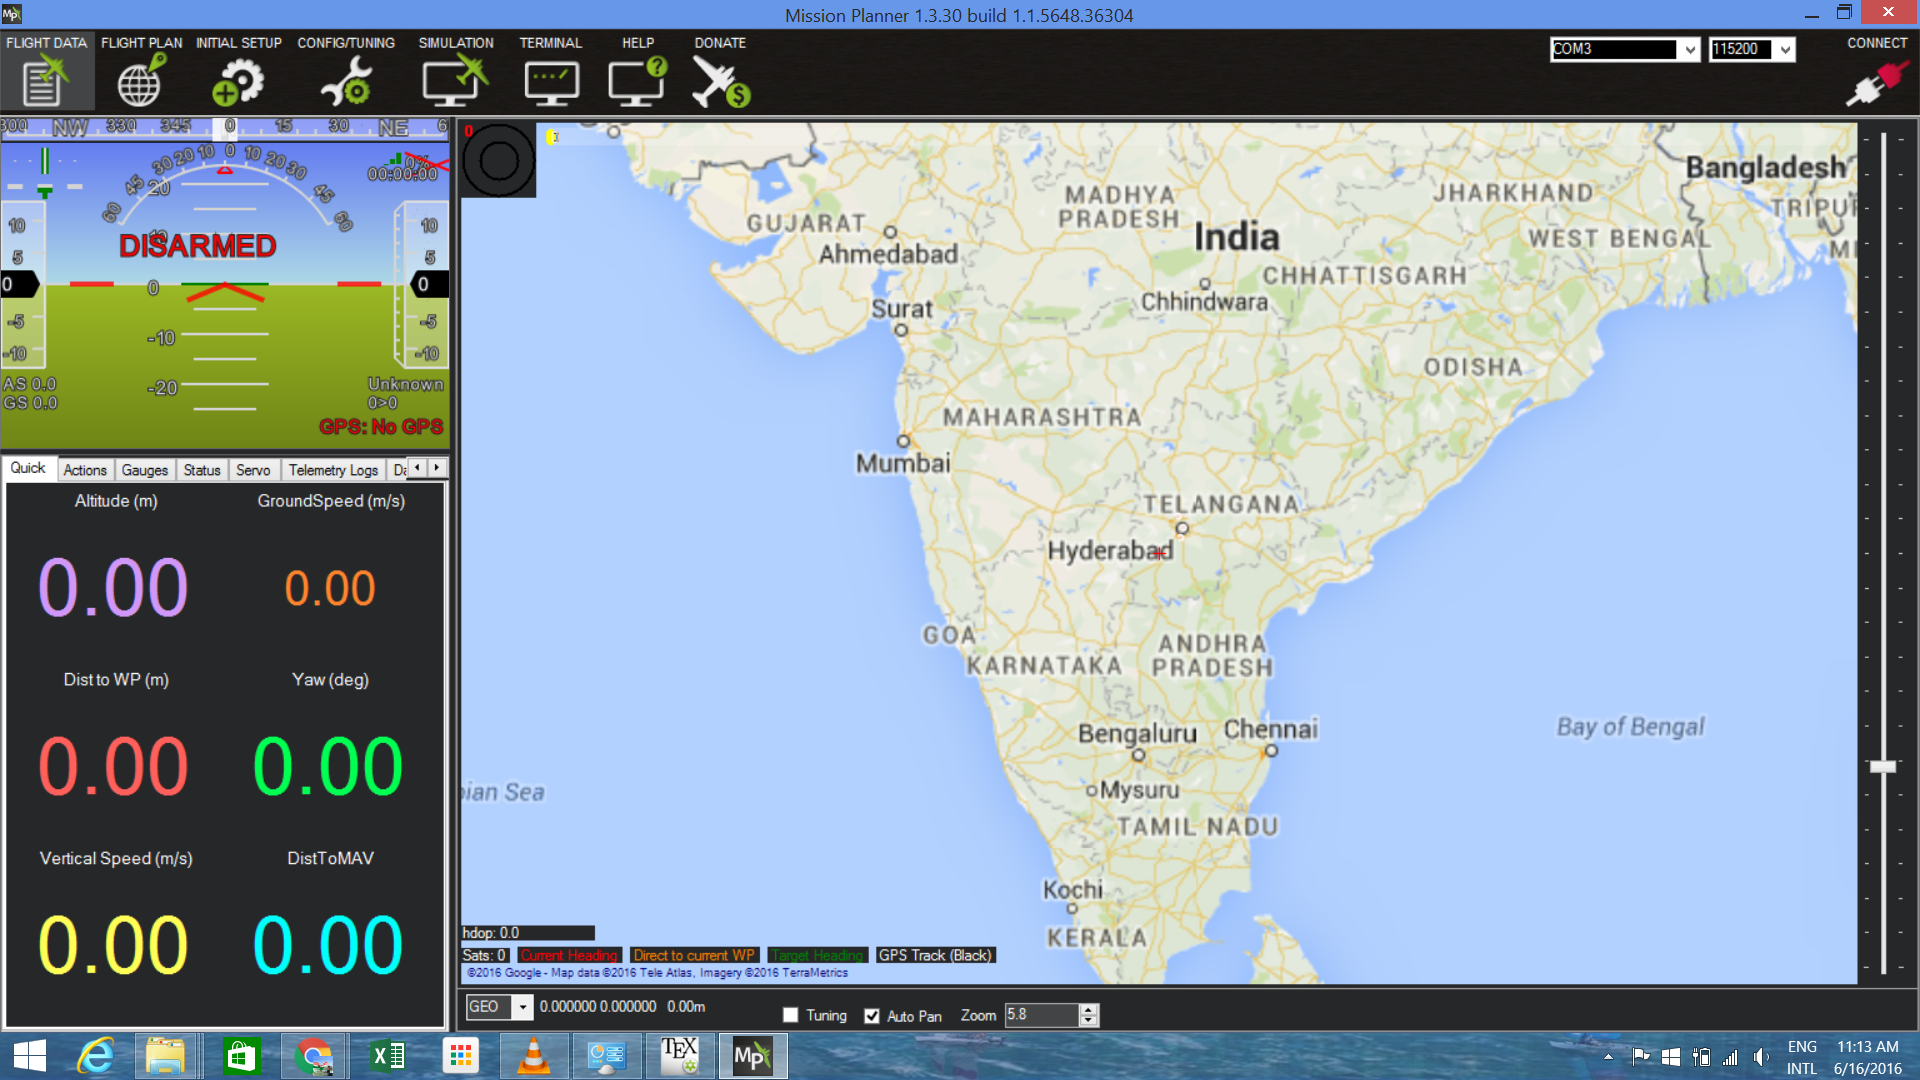
\includegraphics[scale=0.35]{mission}
	 	\caption{Mission Planner.}
\end{figure}
	 \subsection{Installing Mission Planner}
	 The very first step is to install the mission planner software. It is known as GCS or Ground control system. It can be downloaded form here: \url{http://firmware.ardupilot.org/Tools/MissionPlanner/MissionPlanner-latest.msi} \textbf{Note} This link will automatically download the latest version, so if you want to download the previous versions than you can go to \url{http://firmware.ardupilot.org}
	 \paragraph{•}After downloading the software go through the installation process. Follow the instructions to complete the setup process. The installation utility will automatically install any necessary software drivers. If you receive a DirectX installation error, please update your DirectX plug-in from the DirectX Download Center link is: \url{http://www.microsoft.com/en-us/download/details.aspx?id=35}.
	 \paragraph{}If you receive the warning pictured here, select Install this driver software anyway to continue.
	 \begin{figure}[H]
	 	\centering
		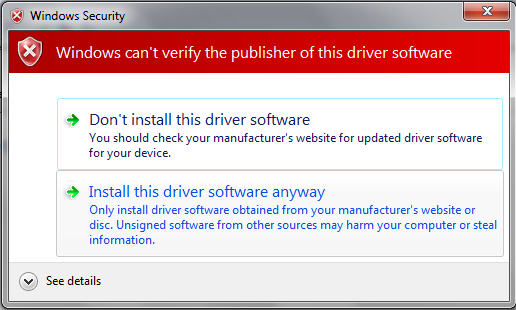
\includegraphics[scale=0.75]{driver}
	 	\caption{Warning Screen.}
\end{figure}

An icon to open the Mission Planner is created according to your instructions during the installation.

	\subsection{Loading Firmware into APM 2.6}
		\subsubsection{Connection}Connect controller to computer
Once you’ve installed the Mission Planner onto your computer, connect the autopilot board to your computer using the micro USB cable as shown below. Use a direct USB port on your computer (not a USB hub).
		\begin{figure}[H]
	 	\centering
		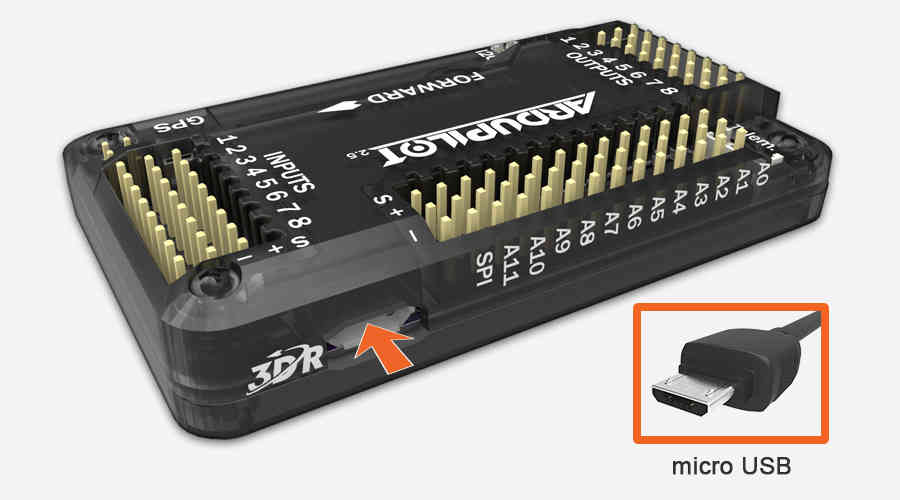
\includegraphics[scale=0.20]{usb}
	 	\caption{APM USB Connection.}
		\end{figure}
		
		\subsubsection{Connect to Mission Planner}
Open the Mission Planner and select the COM port drop-down on the upper-right corner of the screen (near the Connect button). Select AUTO or the specific port for your board (Arduino Mega 2560). Set the Baud rate to 115200 as shown. Don’t hit Connect just yet.
\begin{figure}[H]
	 	\centering
		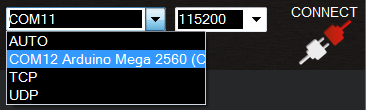
\includegraphics[scale=0.6]{baud}
	 	\caption{COM Port.}
		\end{figure}	
		
		\subsubsection{Install firmware}
On the Mission Planner’s Initial Setup | Install Firmware screen select the appropriate icon that matches your frame (i.e. Quad, Hexa). Answer Yes when it asks you “Are you sure?”.
		\begin{figure}[H]
	 	\centering
		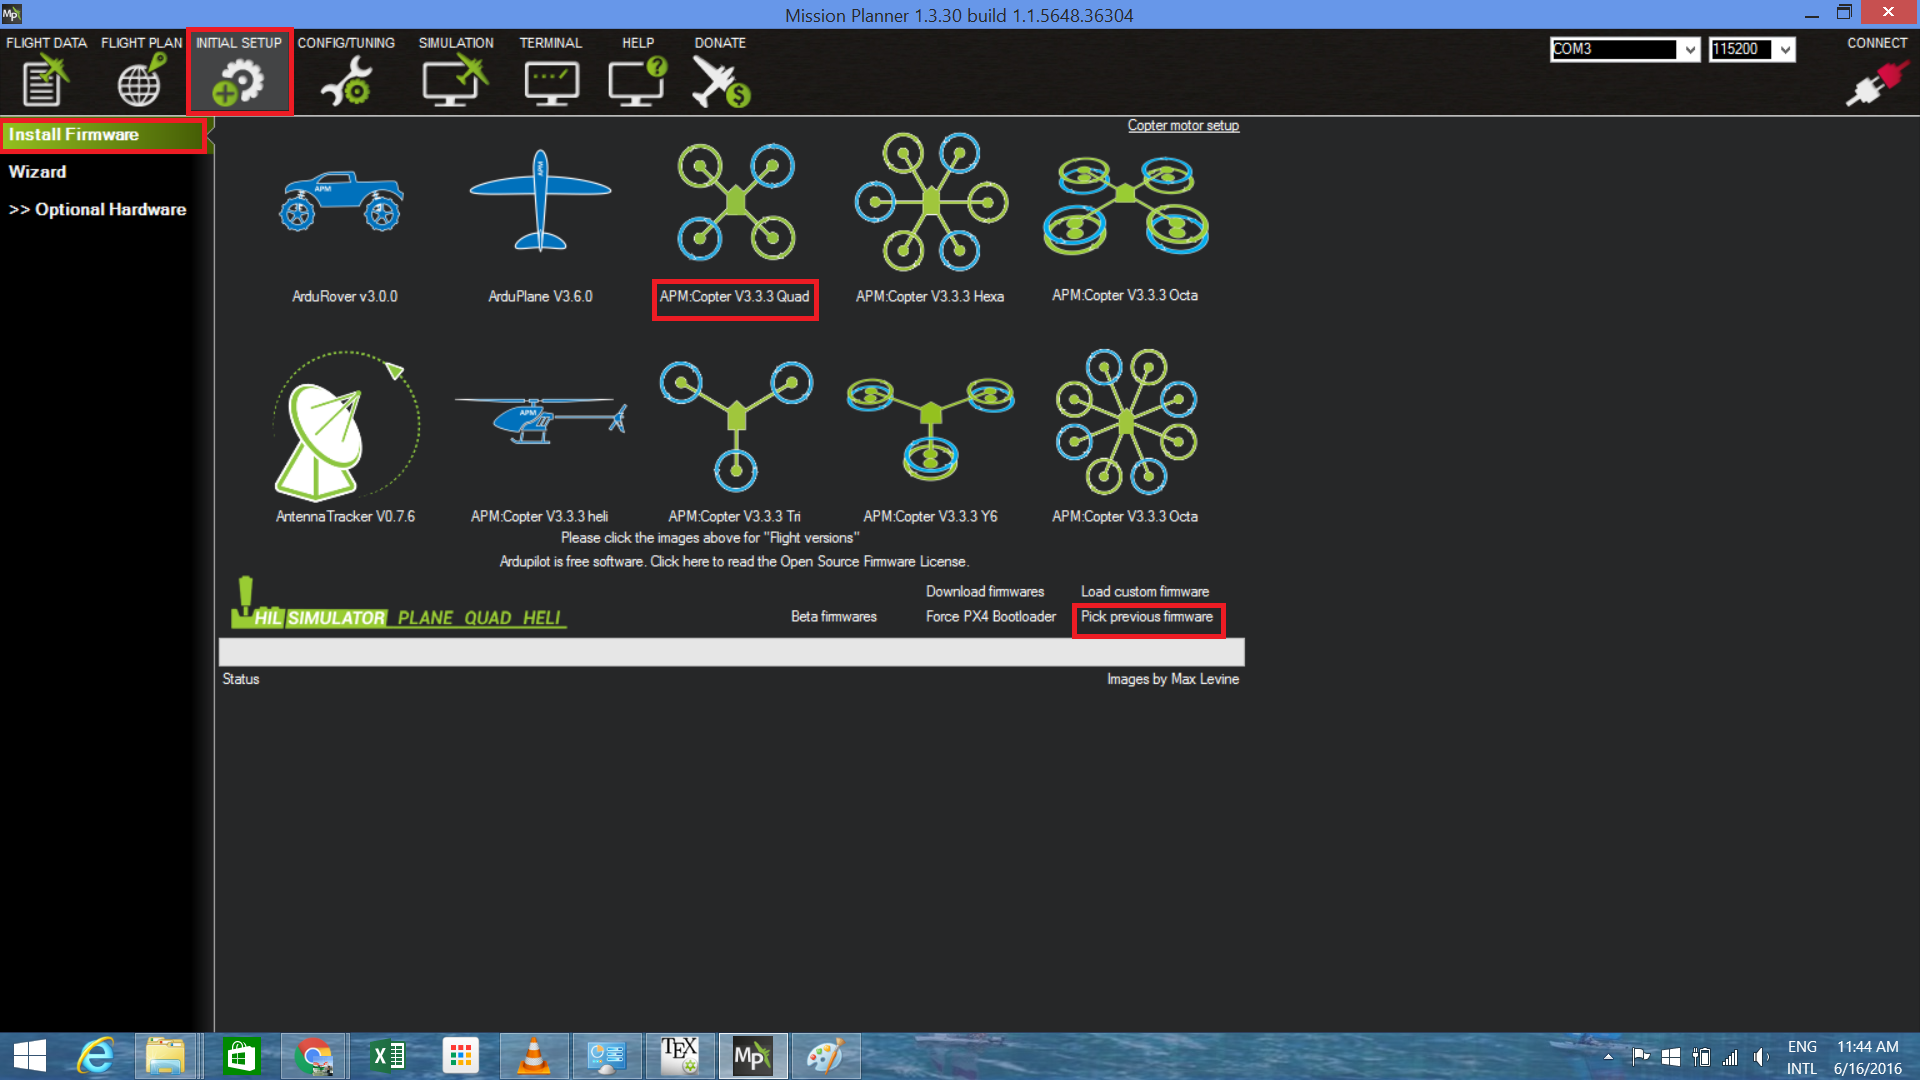
\includegraphics[scale=0.40]{firmware}
	 	\caption{Install Firmware Screen.}
		\end{figure}
		\paragraph{•}Here you will see that the version shown is AC3.3.3 but if you want to use a previous version than you can select pick previous firmware and from the dropdown you can select the required version in this case v3.2.1. If all goes well you will see some status appear on the bottom right including the words, “erase...”, “program...”, “verify..” and “Upload Done”. The firmware has been succesfully uploaded to the board.
		
		\subsection{Calibrating the APM}
			Once you have installed the firmware and if the APM is not connected to the mission planner then click on the connect button on the top right corner. Once the board is connected \paragraph{•} Click on Mandatory Hardware and you will see a dropdown with options like Frame Type, Acc Calibration, etc. Follow the steps in each option and go through the instructions and it should successfully calibrate the APM.
			\paragraph{•} If you need any assistance on how to calibrate then you can check out this link: \url{http://ardupilot.org/copter/docs/configuring-hardware.html} and go through the step by step guide on whole calibration process
		
		\subsection{Testing}
		You can test the firmware is basically working by switching to the Mission Planner Flight Data screen and pressing the Connect button. The HUD should update as you tilt the board.
		
		\subsection{Troubleshooting}
		If Mission planner is unable to connect:

\paragraph{}1. Check that the correct baud rate is used for the selected method (115200 on USB or 57600 on Radio/Telemetry)
\paragraph{}2. If using a COM port on Windows, check that the connection’s COM port exists in the Windows Device Manager’s list of serial ports.
\paragraph{}3. If using a USB port, try a different physical USB port
	\paragraph{}You should also ensure that the autopilot controller board has appropriate ArduPilot firwmare installed and has booted correctly (on APM there are useful LEDs which can tell you the state of the autopilot).
	
	\paragraph{So, if you follow this tutorial properly you should be able to calibrate the APM successfully. You may face some errors like INS not calibrated, Compass/Gyro bad health, RC not calibrated, we suggest that you should go through the process once again and if the error persists then you can find about it's troubleshooting on the net!}
	\section{References}
	\paragraph{•}
	\url{http://ardupilot.org/planner/docs/common-install-mission-planner.html}
	\paragraph{•}\url{http://ardupilot.org/planner/docs/common-loading-firmware-onto-pixhawk.html}
	\paragraph{•}\url{http://ardupilot.org/planner/docs/common-connect-mission-planner-autopilot.html}
	\paragraph{}Everything mentioned above has been referred from the official documentation.
	
\end{document}



